
\documentclass[border=10pt, 12pt]{standalone}
\usepackage[svgnames]{xcolor}
\usepackage{amsmath}
\usepackage{pgfplots}
\pgfplotsset{compat=newest}
\usepackage[sfdefault]{FiraSans}
\usepackage{FiraMono}
\renewcommand*\familydefault{\sfdefault}
\begin{document}
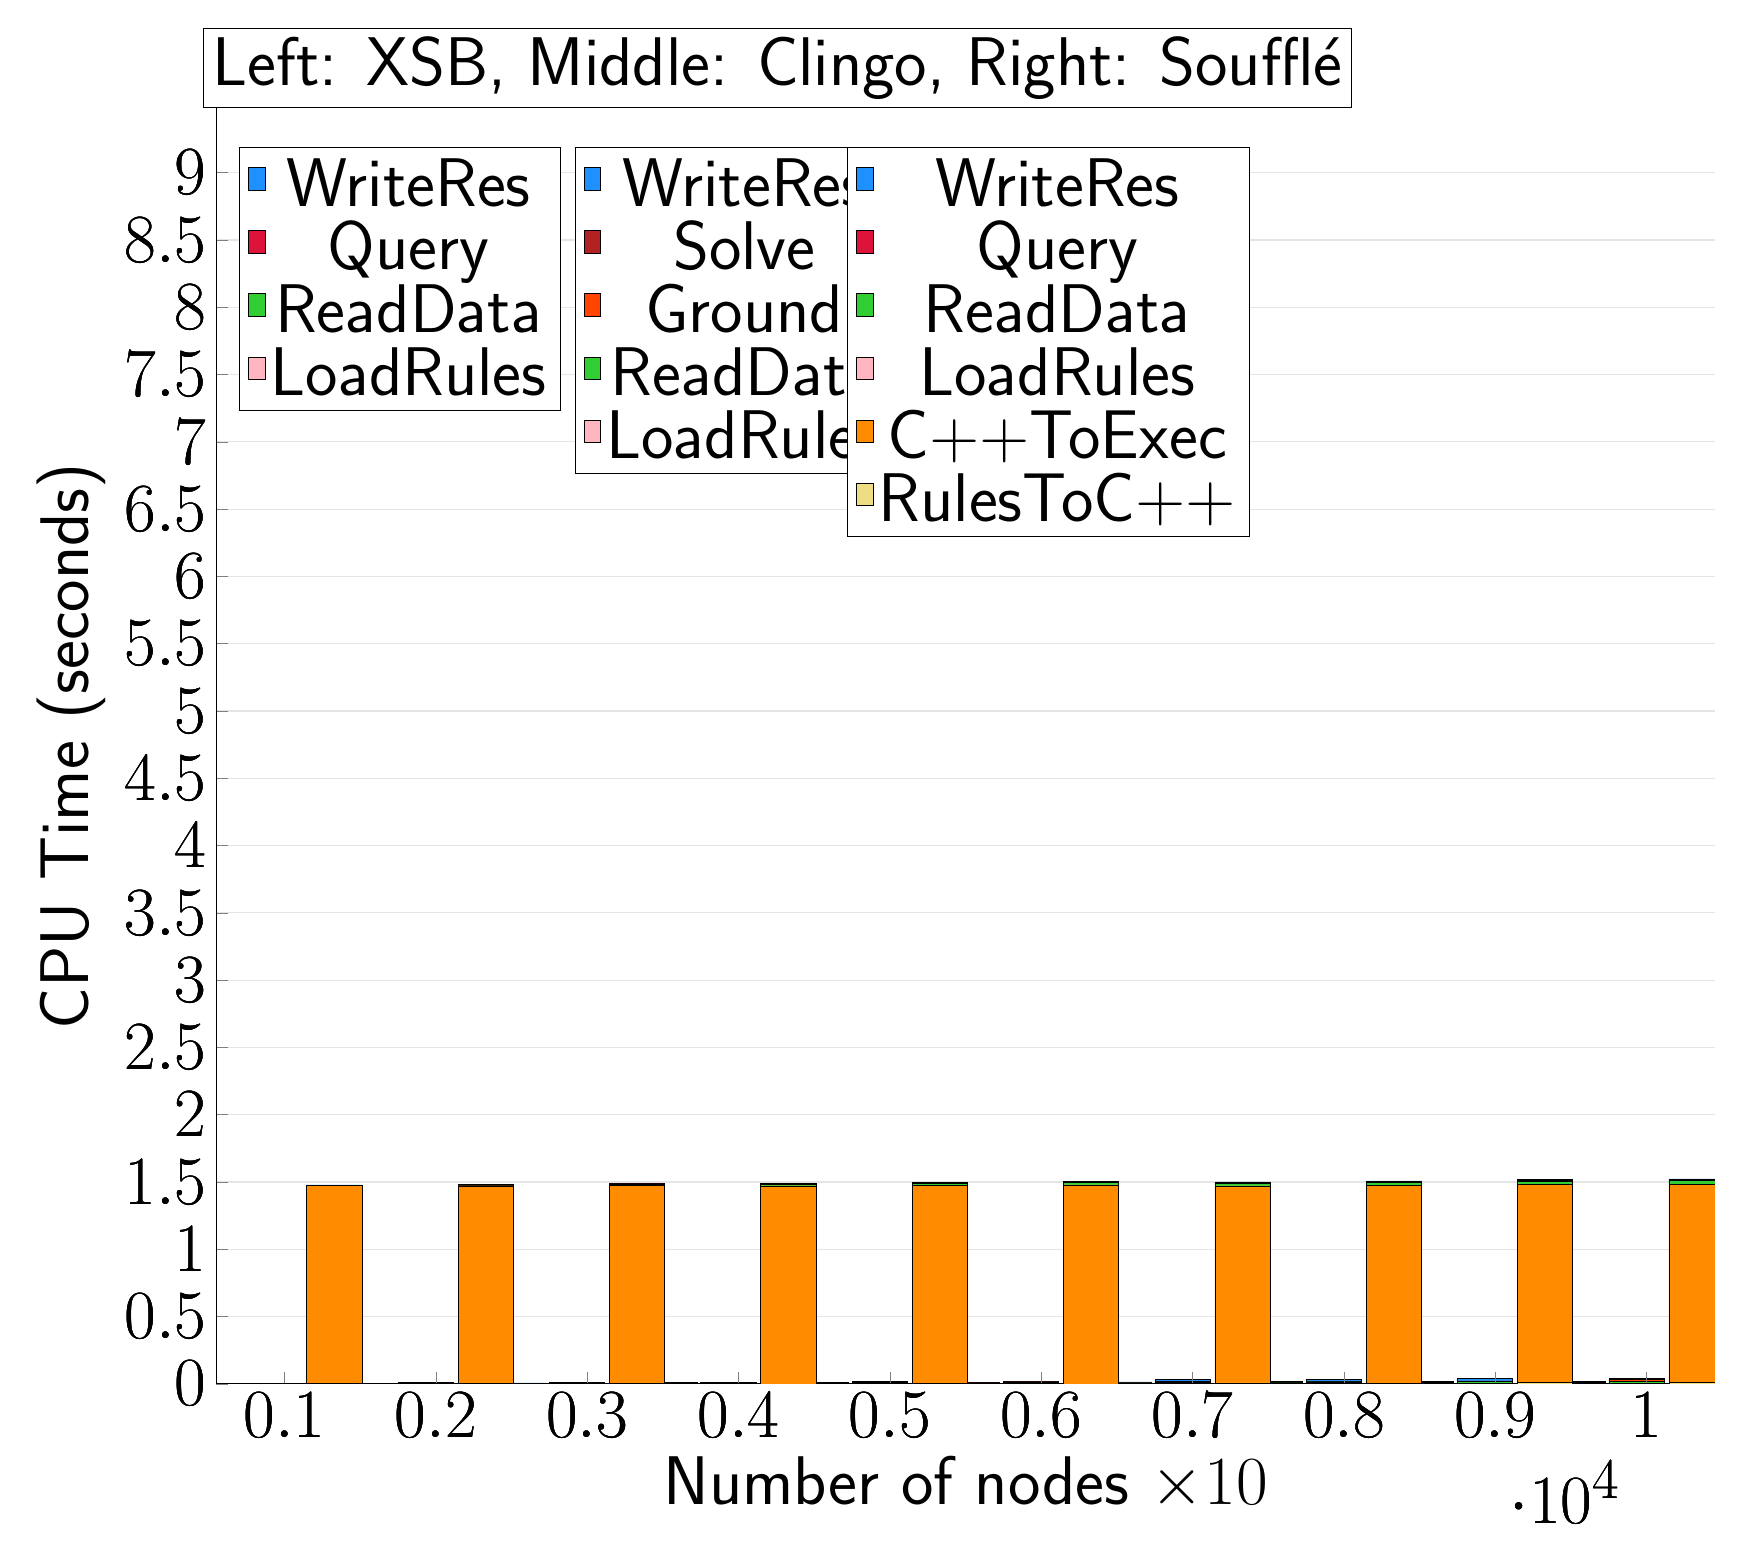
\begin{tikzpicture}
                        \begin{axis}[bar shift=-25pt, 
   ybar stacked,
   width=1.7\textwidth,
   bar width=0.7cm,
   ymajorgrids, tick align=inside,
   major grid style={draw=gray!20},
   xtick=data,
   ymin=0, ymax=9.478,
   axis x line*=bottom,
   axis y line*=left,
   enlarge x limits=0.05,
   legend style={
       at={(0.23, 0.97)},
       anchor=north east,
       legend columns=1,
       font=\Huge,
   },
   ylabel={CPU Time (seconds)},
   xlabel={Number of nodes $\times 10$},
   label style={font=\Huge},
   tick label style={font=\Huge},
]
\addlegendimage{fill=DodgerBlue, draw=black, line width=0.2pt}
\addlegendentry{WriteRes}
\addlegendimage{fill=Crimson, draw=black, line width=0.2pt}
\addlegendentry{Query}
\addlegendimage{fill=LimeGreen, draw=black, line width=0.2pt}
\addlegendentry{ReadData}
\addlegendimage{fill=LightPink, draw=black, line width=0.2pt}
\addlegendentry{LoadRules}
\addplot +[fill=LightPink, draw=black, line width=0.2pt] coordinates {
(1000, 0.0005504)
(2000, 0.0005407999999999999)
(3000, 0.0005493999999999994)
(4000, 0.0005448)
(5000, 0.0005485999999999999)
(6000, 0.0005505999999999999)
(7000, 0.0005470000000000003)
(8000, 0.0005643999999999998)
(9000, 0.0005477999999999999)
(10000, 0.0005480000000000001)
};
\addplot +[fill=LimeGreen, draw=black, line width=0.2pt] coordinates {
(1000, 0.0008896000000000002)
(2000, 0.0016837999999999998)
(3000, 0.0024706)
(4000, 0.0032584000000000003)
(5000, 0.0040464)
(6000, 0.004896599999999999)
(7000, 0.0056974)
(8000, 0.0065632)
(9000, 0.0073114)
(10000, 0.0081772)
};
\addplot +[fill=Crimson, draw=black, line width=0.2pt] coordinates {
(1000, 0.0001511999999999996)
(2000, 0.00029479999999999963)
(3000, 0.0005735999999999998)
(4000, 0.0008057999999999991)
(5000, 0.0010340000000000002)
(6000, 0.0011822)
(7000, 0.0013943999999999998)
(8000, 0.0016184)
(9000, 0.0018432000000000001)
(10000, 0.0019914)
};
\addplot +[fill=DodgerBlue, draw=black, line width=0.2pt] coordinates {
(1000, 0.0009126000000000004)
(2000, 0.0017374000000000005)
(3000, 0.0025764000000000004)
(4000, 0.0033858000000000004)
(5000, 0.004256)
(6000, 0.0050806)
(7000, 0.0059426)
(8000, 0.0068196)
(9000, 0.0075576)
(10000, 0.008365000000000001)
};
\end{axis}

\begin{axis}[bar shift=-3.7pt, 
   ybar stacked,
   width=1.7\textwidth,
   bar width=0.7cm,
   ymajorgrids, tick align=inside,
   major grid style={draw=none},
   xtick=data,
   ymin=0, ymax=9.478,
   axis x line*=none,
   axis y line*=none,
   enlarge x limits=0.05,
   legend style={
       at={(0.454, 0.97)},
       anchor=north east,
       legend columns=1,
       font=\Huge,
   },
   label style={font=\Huge},
   tick label style={font=\Huge},
]
\addlegendimage{fill=DodgerBlue, draw=black, line width=0.2pt}
\addlegendentry{WriteRes}
\addlegendimage{fill=FireBrick, draw=black, line width=0.2pt}
\addlegendentry{Solve}
\addlegendimage{fill=OrangeRed, draw=black, line width=0.2pt}
\addlegendentry{Ground}
\addlegendimage{fill=LimeGreen, draw=black, line width=0.2pt}
\addlegendentry{ReadData}
\addlegendimage{fill=LightPink, draw=black, line width=0.2pt}
\addlegendentry{LoadRules}
\addplot +[fill=LightPink, draw=black, line width=0.2pt] coordinates {
(1000, 0.0)
(2000, 0.0)
(3000, 0.0)
(4000, 0.0)
(5000, 0.0)
(6000, 0.0)
(7000, 0.0)
(8000, 0.0)
(9000, 0.0)
(10000, 0.0)
};
\addplot +[fill=LimeGreen, draw=black, line width=0.2pt] coordinates {
(1000, 0.0)
(2000, 0.0)
(3000, 0.0020000000000000018)
(4000, 0.008000000000000007)
(5000, 0.010000000000000009)
(6000, 0.010000000000000009)
(7000, 0.01200000000000001)
(8000, 0.014000000000000012)
(9000, 0.020000000000000018)
(10000, 0.020000000000000018)
};
\addplot +[fill=OrangeRed, draw=black, line width=0.2pt] coordinates {
(1000, 0.0)
(2000, 0.0)
(3000, 0.008000000000000007)
(4000, 0.0020000000000000018)
(5000, 0.0)
(6000, 0.0040000000000000036)
(7000, 0.008000000000000007)
(8000, 0.006000000000000005)
(9000, 0.0020000000000000018)
(10000, 0.010000000000000009)
};
\addplot +[fill=FireBrick, draw=black, line width=0.2pt] coordinates {
(1000, 0.0)
(2000, 0.0)
(3000, 0.0)
(4000, 0.0)
(5000, 0.0)
(6000, 0.0040000000000000036)
(7000, 0.0)
(8000, 0.0)
(9000, 0.0)
(10000, 0.0)
};
\addplot +[fill=DodgerBlue, draw=black, line width=0.2pt] coordinates {
(1000, 0.0)
(2000, 0.008000000000000007)
(3000, 0.0)
(4000, 0.0020000000000000018)
(5000, 0.010000000000000009)
(6000, -0.0020000000000000018)
(7000, 0.010000000000000009)
(8000, 0.010000000000000009)
(9000, 0.016000000000000014)
(10000, 0.010000000000000009)
};
\end{axis}

\begin{axis}[bar shift=18pt, 
   ybar stacked,
   width=1.7\textwidth,
   bar width=0.7cm,
   ymajorgrids, tick align=inside,
   major grid style={draw=none},
   xtick=data,
   ymin=0, ymax=9.478,
   axis x line*=none,
   axis y line*=none,
   enlarge x limits=0.05,
   legend style={
       at={(0.69, 0.97)},
       anchor=north east,
       legend columns=1,
       font=\Huge,
   },
   label style={font=\Huge},
   tick label style={font=\Huge},
]
\addlegendimage{fill=DodgerBlue, draw=black, line width=0.2pt}
\addlegendentry{WriteRes}
\addlegendimage{fill=Crimson, draw=black, line width=0.2pt}
\addlegendentry{Query}
\addlegendimage{fill=LimeGreen, draw=black, line width=0.2pt}
\addlegendentry{ReadData}
\addlegendimage{fill=LightPink, draw=black, line width=0.2pt}
\addlegendentry{LoadRules}
\addlegendimage{fill=DarkOrange, draw=black, line width=0.2pt}
\addlegendentry{C++ToExec}
\addlegendimage{fill=LightGoldenrod, draw=black, line width=0.2pt}
\addlegendentry{RulesToC++}
\addplot +[fill=LightGoldenrod, draw=black, line width=0.2pt] coordinates {
(1000, 0.0020000000000000005)
(2000, 0.0020000000000000005)
(3000, 0.0020000000000000005)
(4000, 0.0)
(5000, 0.004000000000000001)
(6000, 0.0)
(7000, 0.006000000000000001)
(8000, 0.004000000000000001)
(9000, 0.008000000000000002)
(10000, 0.010000000000000002)
};
\addplot +[fill=DarkOrange, draw=black, line width=0.2pt] coordinates {
(1000, 1.4700000000000002)
(2000, 1.4679999999999997)
(3000, 1.47)
(4000, 1.47)
(5000, 1.47)
(6000, 1.4780000000000002)
(7000, 1.464)
(8000, 1.472)
(9000, 1.476)
(10000, 1.4740000000000002)
};
\addplot +[fill=LightPink, draw=black, line width=0.2pt] coordinates {
(1000, 0.000162)
(2000, 0.0001806)
(3000, 0.0001718)
(4000, 0.0001794)
(5000, 0.00016519999999999998)
(6000, 0.00017039999999999997)
(7000, 0.00017500000000000003)
(8000, 0.0001654)
(9000, 0.00016079999999999998)
(10000, 0.000172)
};
\addplot +[fill=LimeGreen, draw=black, line width=0.2pt] coordinates {
(1000, 0.0037700000000000003)
(2000, 0.0067308)
(3000, 0.009420000000000001)
(4000, 0.0126858)
(5000, 0.014588399999999998)
(6000, 0.0162232)
(7000, 0.0187934)
(8000, 0.0195762)
(9000, 0.021140399999999997)
(10000, 0.025245200000000002)
};
\addplot +[fill=Crimson, draw=black, line width=0.2pt] coordinates {
(1000, 0.001434)
(2000, 0.0025512)
(3000, 0.0040978)
(4000, 0.0049254)
(5000, 0.0061042)
(6000, 0.007317800000000001)
(7000, 0.008381)
(8000, 0.008890200000000001)
(9000, 0.0089306)
(10000, 0.010400200000000002)
};
\addplot +[fill=DodgerBlue, draw=black, line width=0.2pt] coordinates {
(1000, 0.0008460000000000001)
(2000, 0.0013428)
(3000, 0.0017036)
(4000, 0.0020724)
(5000, 0.0023284)
(6000, 0.0025958)
(7000, 0.0027987999999999997)
(8000, 0.0029826)
(9000, 0.0031342)
(10000, 0.0034005999999999993)
};
\end{axis}


\node[anchor=south, draw, fill=white] at (rel axis cs:0.42,1) {\Huge Left: XSB, Middle: Clingo, Right: Soufflé};
\end{tikzpicture}
\end{document}
                    